\chapter{Reporting Power Values \normalsize{(Detailed Information)}}
\label{sec:reporting}

\noindent
This section describes the information that must be included with a power measurement submission. It also describes some optional information that submitters may decide to include.
\wl

\noindent
The section contains definitions of the terms used to describe the elements of a power submission, some background information, motivation about why the list contains the elements it does, and any other details that may be helpful.
\noindent


\section{Measuring Device Specifications}
\label{sec:MDSpecs}
\noindent
Measuring devices must meet the Level requirements as defined in 
Sections~\ref{sec:AQLevels} and \ref{sec:A1GTRM}. This section defines meter accuracy requirements.
\wl

\noindent
For Level~3, it is required to use any revenue grade meter, any meter accepted by spec power, or any meter documented to have an accuracy of 1\% or better. 
Level~2 requires a meter with a minimum documented accuracy of 2\%.
Level~1 requires a meter with a minimum documented accuracy of 5\%.
\wl

\noindent
The required accuracy as percentage refers to the relative error specified for the power meter.
If the power meter has multiple measurement intervals with different accuracies, all measurement intervals used during the benchmark run must meet the above requirements.
Error in this context refers to the sum of statistical and systematic error.
It is acceptable if the error is documented either as a hard bound, as the 1$\sigma$ standard deviation, or as the full width at half maximum (FWHM).
\wl

\noindent
If the site uses multiple independent power meters for a Level~2 or a Level~3 measurement, and if all employed power meters measure an identical fraction of the system, the requirements are relaxed in the following way.
\begin{packed_item}
\item 
Each individual power meter must have at least a documented accuracy of 3\%.
\item
The documented error of the individual meters divided by the square root of the number of employed meters must meet the above requirements of 2\% for Level~2 and 1\% for Level~1.
\end{packed_item}
In this case, the second requirement ensures that the standard deviation of the measurement of the entire run, using error propagation, and assuming a gaussian distribution, and assuming that the errors of the power meters are uncorelated, meets the requirements.
For example, assume 4 power meters for a Level~3 measurement, each measuring 25\% of the total system.
In that case, each meter must have a documented accuracy of~$1\% \cdot \sqrt{4} = 2\%$.
In other words, you can use a single meter with 1\% accuracy, 4 meters with 2\% accuracy, or 9 meters with 3\% accuracy for Level~3.
\wl

\noindent
Revenue grade meters are defined by ANSI C12.20.
For meters accepted by the spec power, refer to the {\itshape Power and Temperature Measurement Setup Guide \/} and the list of accepted power measurement devices from the Standard Performance Evaluation Corporation.
\begin{packed_item}
\item 
\url{http://www.spec.org/power_ssj2008/}
\item
\url{http://www.spec.org/power/docs/SPECpower-Device_List.html }
\end{packed_item}
\wl

\section{Measuring Device Terminology}
\label{sec:MDTerm}
\noindent
Levels 1 and 2 specify power measurements. Level~3 specifies an energy measurement, but reports a power value.

\subsection{Sampling and Power Readings}
\noindent
For Levels 1 and 2, the power meter must internally sample the instantaneous power at a constant frequency of at least once per second.
(Internally, one such power sample will usually require many more measurements of voltage and current taken much more frequently than once per second.
The power meter will either integrate the measurements at a high frequency, or fit a sine wave curve to it and determine the power factor and in this way produce a power consumption reading.)
Usually the net frequency varies by a small percentage around 50~Hz or 60~Hz.
It is allowed that the measurement sample frequency is not strictly constant, but it can be adjusted such that each sample interval covers a certain number of full sine waves.
In that case, the intervals must not exceed one second by more than one sine wave and when building the final power average the power readings must be weighted by the duration of the sample interval.
\wl

\noindent
Sampling in an AC context requires a measurement stage that determines the true power delivered at that point and enters that value into a buffer where it is then used to calculate average power over a longer time.  So ``sampled once per second'' in this context means that the times in the buffer are averaged and recorded once per second.
Sampling delivered electrical power in a DC context refers to a single simultaneous measurement of the voltage and the current to determine the delivered power at that point.  The sampling rate in this case is how often such a sample is taken and recorded internally within the device.  
\wl

\noindent
If the submitter is sampling in a DC context, most likely it will be necessary to adjust for power loss in the AC/DC conversion stage. 
Refer to Section~\numnameref{sec:A3SIiIP} for details.
\wl

\noindent
It is allowed that the power meter does not report every sample.
Instead, the power meter may use an internal buffer and aggregate several samples over time and then only report one average power reading at a certain constant frequency.
In the following, we refer to such a reported power measurement of the power meter as ``power reading''.
The intervals between the power readings must be no longer than 10\% of the duration of the core phase.
If the power meter reports every sample, then a power sample and a power reading is the same.
\wl

\noindent
The power meter must use all power samples taken during an interval to compute the average power reading.
Consider that the limits of one sample per second and one power reading per 10 seconds / 1 minute are upper bounds.
Usually, the power meter will take many samples per second and report power readings on about a per second basis.

\subsection{Power-Averaged and Total Energy Measurements}
\label{sec:PAaTEM}

This subsection describes the difference of power-averaged measurements as required for Level~1 and Level~2 as compared to total energy measurements as required for Level~3.

\subsubsection{Power-Averaged Measurements}

\noindent
The reported power values for Levels 1 and 2 are power-averaged measurements over a certain time period (e.g. the core phase or the full run).
A power-averaged measurement is one taken by a device that samples the instantaneous power used by a system at some fine time resolution for a specified interval.
This interval is short compared to the full time of the power-averaged measurement.
The power meter device numerically averages of all the instantaneous power measurements sampled during that interval.
This constitutes one measurement reported by the device covering that interval.
Finally, the power-averaged measurement for the required time period is the average of all these power readings obtained from the device in that period.
All power readings reported by the device for that period must be used except for one case:
Exclude those readings for intervals that do not lie completely in the requested time period.
(Usually the reading intervals and the measured time period (e.g. the core phase) are not synchronized.)
We require that the internal device sampling rate must be at least 1 Hz and constant.
The intervals between the power readings must be constant and no longer than 10\% of the duration of the core phase.
(This ensures that the parts of the core phase that are not measured at beginning and end are not significant.)
As noted in the previous subsection, the sampling rate may vary slightly to accomodate for variations in the net frequency.
In that case, the averaging process must weight the power readings from the power meter according to the respective interval lengths.
\wl

\noindent
Consider Level~1, which requires only one reported power value. 
This reported power value may consist of several power readings taken at a constant frequency of at least once per minute.
Each such reading itself must be the average of instantaneous power samples measured at least once per second and averaged over reading interval.
For Level~1, the time period that is measured must be the core phase of the run, which must be at least one minute long (see \ref{sec:core_phase} for definition of core phase).
For example, if the device reports one power measurement every 5 seconds (each being the average of at least 5 power samples) and the core phase takes 10 minutes, Level~1 reports one power-averaged value that averages over all the 120 measurements obtained during the core phase.
(Usually the power reading intervals and the core phase are not synchronized, such that the first reding does not lie completely in the core phase. In that case the average is only over the 119 readings completely in the core phase.)
\wl

\noindent
Level~2 also requires that power measurements be taken at a constant frequency and the device must internally sample internally at least once per second.
It requires the submission of the power-averaged measurement for the core phase, for the full run, and for a series of equally spaced power-averaged measurements of equal length during the full run.
These power-averaged measurements in the series must be spaced close enough so that at least 10 measurements are reported during the core phase of the workload.
There must not be any delay between the power measurement in this series and they must cover the entire core phase.
Alternatively, instead of the 10 power-averaged measurements, it is allowed to submit the full set of power readings from the device that are used to calculate the average power during the core phase and during the full run.
\wl

\noindent
The measurement for the core phase for Level~2 is identical to the measurement in Level~1.
Assume again one measurement every 5 seconds (consisting of 5 samples each), a core phase of 10 minutes and a full run of 15 minutes.
In that case, the submission includes one power-averaged measurement over 120 power readings for the core phase, one power-averaged measurement over 180 readings for the full run, and for instance a series of 30 power-averaged measurements over 6 power readings each, once every 30 seconds.
\wl

\noindent
For Levels 1 and 2, the units of the reported power values are watts.
\wl

\subsubsection{Total Energy Measurements}

\noindent
Level~3 specifies a total energy measurement that, when divided by the measured time, also reports power. An integrated measurement is a continuing sum of energy measurements. Typically, there are hundreds of measurements per second.  Depending on the local AC power line frequency, there must be at least 120 or 100 measurements per second. The measuring device samples voltage and current many times per second and integrate those samples to determine the next total energy consumed reading. 
\wl

\noindent
Level~3 reports an average power value for the core phase, an average power value for the whole run, at least 10 equally spaced energy values within the core phase, and the elapsed times between the first and last energy readings in both the core phase and the full run.
These last and first measurements in the core phase must be timed such that no more than a total of ten seconds (five each at begin and end) of the core phase are not covered by the total energy measurement.
The final average power value for the core phase is the difference between the first and last energy readings divided by the elapsed time between first and last reading.
The final value for the full run must be obtained analogously.
\wl

\noindent
The difference between the initial and final energy readings are the total energy measurement in joule. The reported values after the energy has been divided by the elapsed time are watts as for levels 1 and 2.

\section{Aspect and Quality Levels}
\label{sec:AQLevels}
\noindent
Table~\ref{tab:levels} summarizes the aspect and quality levels introduced in Section~\ref{sec:intro} Introduction

%INSERT TABLE 1
\noindent
\begin{table}
\caption{Summary of aspects and quality levels}
\label{tab:levels}
\begin{tabular}{|p{3.0cm}|p{3.5cm}|p{3.5cm}|p{3.5cm}|} \hline
\textbf{Aspect}&\textbf{Level~1}&\textbf{Level~2}&\textbf{Level~3}\\ \hline

\textbf{1a:~Granularity} &
One power sample per second &
One power sample per second &
Continuously integrated energy\\
\hline


\textbf{1b:~Timing} &
The entire core phase of the run, at least one minute &
At equal intervals across the full run &
At equal intervals across the full run   \\
\hline

\textbf{1c:~Measurements} &
Core phase average power &
$\bullet$ Core phase average power & 
$\bullet$ Core phase total energy \\MDSpecs

 & &
$\bullet$ Full run average power &
$\bullet$ Full run total energy \\

 & &
$\bullet$ 10 average power measurements in the core phase &
$\bullet$ 10 total energy measureMDSpecsments in the core phase \\

 & &
$\bullet$ idle power &
$\bullet$ idle power \\
\hline

\textbf{2: Machine \newline fraction}  &
The greater of 1/10 of the compute subsystem or 2~kW or 15~compute nodes. Alternatively at least 40~kW or the entire system. &
The greater of 1/8 of the compute-node subsystem or 10~kW or 15~compute nodes &
The whole of all included subsystems \\
\hline

\textbf{3:~Subsystems} &
Compute-nodes measured, interconnect measured or estimated &
Compute-nodes measured, all participating subsystems measured or estimated &
All participating subsystem must be measured \\
\hline

\textbf{4: Location of measurement} &
Upstream of power conversion &
Upstream of power conversion &
Upstream of power conversion\\

 &
\centering \textbf{OR} &
\centering \textbf{OR} &
\centering \textbf{OR} \tabularnewline

 &
Conversion loss modeled with manufacturer data &
Conversion loss modeled with off-line measurements of a single power supply &
Conversion loss measured simultaneously \\
\hline
\textbf{4b: Meter accuracy} &
5\% &
2\% (see Section~\ref{sec:MDSpecs})&
1\% (see Section~\ref{sec:MDSpecs})\\
\hline
\end{tabular}
\end{table}

\section{Aspect 1: Granularity, Timespan and Reported Measurements}
\label{sec:A1GTRM}
\noindent
Aspect 1 has the following three parts. Levels 1, 2, and 3 satisfy this aspect in different ways.

\begin{itemize}
\item
The granularity of power measurements. This aspect determines the number of measurements per time element.
\item
The timespan of power measurements. This aspect determines where in the time of the workload's execution the power measurements are taken.
\item
The reported measurements. This aspect describes how the power measurements are reported.
\end{itemize}

\noindent
For all required measurements, the submission must also include the data used to calculate them. For Level~2 and Level~3 submissions, the supporting data must include at least 10 measurement values at a regular sampling rate in the core phase of the run. 
\wl

\noindent
Levels 2 and 3 require reported measurement values at regular intervals for the following reasons:

\begin{itemize}
\item
Facility or infrastructure level power measurements are typically taken by a system separate from the system OS and thus cannot be easily synchronized with running the benchmark.
\item
With multiple periodic measurements, more measurement values are included before and after the benchmark run.
This ensures that a uniform standard of \textit{beginning} and \textit{end} of the power measurement can be applied to all the power measurements from different sensors.
\end{itemize}

\noindent
There is no maximum number of reported measurement values, although one reported measurement per second is a reasonable upper limit. The submitter may choose to include more than 10 such measurement values.
\wl

\noindent
The number of reported average power measurements or total energy measurements is deliberately given large latitude.  Different computational machines will run long or short benchmark runs, depending on the size of the machine, the memory footprint per node, as well as other factors.  Typically the power measurement infrastructure is not directly tied to the computational system's OS and has its own baseline configuration (say, one averaged measurement every five minutes).  These requirements are specified not only to give a rich data set but also to be compatible with typical data center power measurement infrastructure.
\wl

\noindent
All levels specify that power measurements be performed within the core phase of a workload. Levels 2 and 3 specify that a power measurement for the entire application be reported. Consequently, these levels require measurements during the run but outside of the core phase.

\subsection{Core Phase}
\label{sec:core_phase}
\noindent
All submissions must include the average power within the core phase of the run. 
\wl

\noindent
The core phase is usually considered to be the section of the workload that undergoes parallel execution. 
It typically does not include the parallel job launch and teardown and is required to run for at least one minute.
\wl

\noindent
In order to correlate the power measurement and the performance measurement to obtain the power efficiency, power and performance must be measured over the exact same time period.
Therefore, the core phase is defined as the time period that is used for the performance calculation.
Sometimes, the exact same time is impossible to measure due to power meter restrictions.
Therefore, Level~1 and Level~2 allow a small part at the beginning and at the end which is not measured (see Section~\ref{sec:PAaTEM}).
\wl

\noindent
For example, the core phase of the Linpack workload is the portion of the code that actually solves the matrix.
It is the numerically intensive solver phase of the calculation.
In case of the standard HPL implementation of the Linpack benchmark as provided by netlib.org (\url{http://www.netlib.org/benchmark/hpl/}) this is the time spent in the routing {\ttfamily HPL\_pdgesv}.
Note that HPL as of version 2.1 contains a timer routine that prints start and end time of the core phase to facilitate power measurements, which looks like:\newline
{\ttfamily
HPL\_pdgesv() start time Wed Jun 30 21:49:08 2015\newline
HPL\_pdgesv() end time Wed Jun 30 22:23:15 2015
}.

\subsection{The Whole Run}
\noindent
Level~2 and Level~3 submissions must also include the average power for the whole run, from the initiation of the job to its completion. 
\wl

\noindent
Since HPL only reports the time spent executing the core phase of the workload, the time for the total run must be measured and reported separately by the submitter, for example by prepending the UNIX time command to the job invocation or the parallel application launch, whichever is earlier.
\wl

\noindent
Levels 2 and 3 require the entire run to be measured and reported because HPL (the default workload at the time this document was written) drops significantly in power consumption during the course of a computation, as the matrix size being computed gets smaller.  Requiring the entire run eliminates systematic bias caused by using different parts of the run for the measurement. Figure~\ref{fig:powprof} shows an example of a power graph taken from an HPL run on the LLNL Muir system in the fall of 2011.
\wl

\noindent
Note that the power drops by 8\% or so during the computational phase of the run.  This graph also illustrates the need for the device measurement to have as high a time resolution as possible.  The spread of power measurements even within a small time span is very likely caused by the sampling going in and out of phase with the AC input power. Figure~\ref{fig:sopm} shows a smaller time slice that clearly illustrates this.
\wl


%INCLUDE FIG 3-1
\begin{figure}
\centering
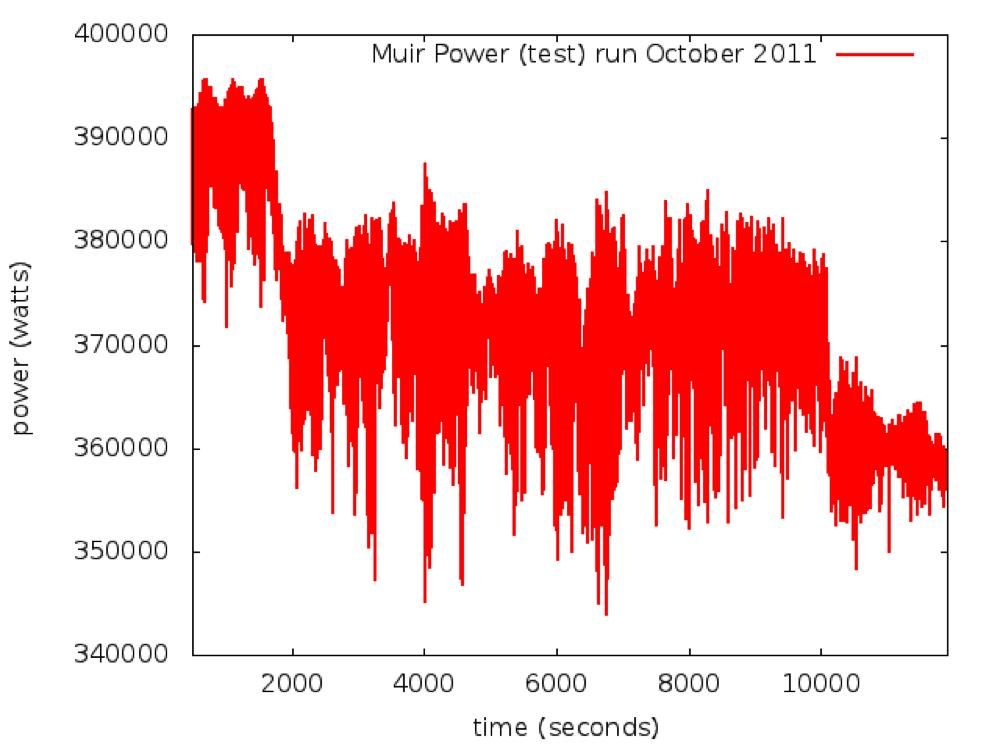
\includegraphics[width=4in]{fig3-1}
\caption{Power Profile HPL Run}
\label{fig:powprof}
\end{figure}

%INCLUDE FIG 3-2
\begin{figure}
\centering
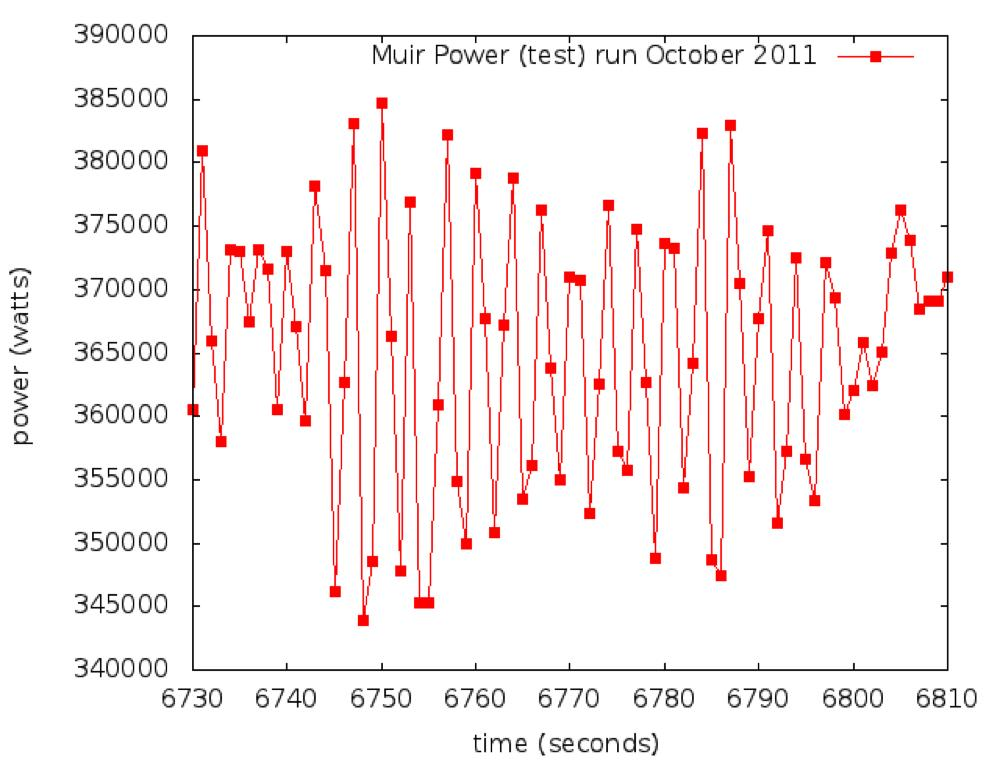
\includegraphics[width=4in]{fig3-2}
\caption{Spread of Power Measurements}
\label{fig:sopm}
\end{figure}

\noindent
The boxes are individual one-second power samples.  This fast up-down fluctuation is not caused by the behavior of an individual power supply; the power being sampled is over the entire computer system doing the HPL run.  The reason that L3 requires integrating total energy meters is because they measure at a high enough sampling rates to not be subject to these sampling artifacts.
\wl

\noindent
L3 requires a power-meter device with a higher inherent measurement granularity as compared to L1 and L2.
L1 / L2 allow 1-second intervals of the input power.
L3 requires an integrating total-energy meter, which samples the input power multiple times per AC cycle and so is much less susceptible to sampling artifacts caused by the AC waveform.  

\subsection{Level~1}
\noindent
The device measurement granularity must be at least one instantaneous measurement of power per second. This requirement holds whether the measurement is DC or AC.
\wl

\noindent
There must be at least one power-averaged measurement during the run.
The total interval covered must be the core phase of the run which must be at
least one minute long.
\wl

\subsection{Level~2}
\noindent
Level~2 submissions include a measurement of the average power during the core phase of the run and the average power during the full run. The workload run must have a series of power-averaged measurements at constant time intervals. These measurement intervals must be short enough so that at least 10 measurements are reported during the core phase of the workload. The reported average power for the core phase of the run will be the numerical average of the 10 (or more) power-averaged measurements collected during the core phase.  
\wl

\noindent
The complete set of power-averaged measurements used to calculate average power must also be provided.
The device measurement sampling granularity must be at least one instantaneous measurement of power per second.
\wl

\noindent
There is some unspecified number of power-averaged measurements during the workload but outside of the core phase. The reported average power for the whole run will be the numerical average of the power measurements for the whole run.  
\wl


\noindent
Figure~\ref{fig:a1l2pm} illustrates Aspect~1 of a Level~2 power measurement. Each measurement is an average of instantaneous power measurements, and these instantaneous measurements are taken once per second. As an example, the figure shows 10 power-averaged measurements within the core phase and four power-averaged measurements outside the core phase, two before the core phase and two after the core phase.

%INCLUDE FIG 3-4
\begin{figure}
\centering
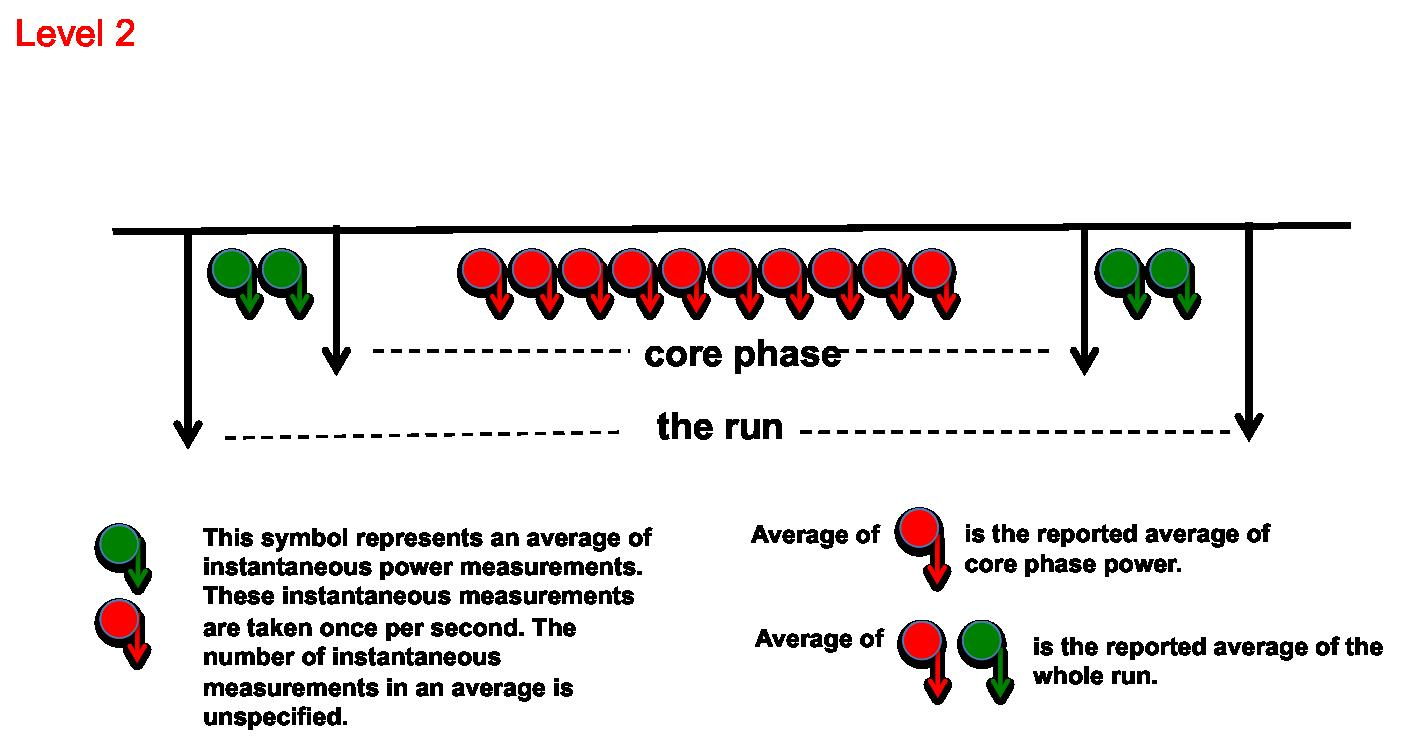
\includegraphics[width=4in]{fig3-4}
\caption{Aspect~1 of Level~2 Power Measurements}
\label{fig:a1l2pm}
\end{figure}

\subsection{Level~3}
\noindent
Level~3 submissions include a measurement of the average power during the core phase of the run and the average power during the full run.
\wl

\noindent
The complete set of total energy readings (at least 10 during the core computation phase) must be included, along with the execution time for the core phase and full run. 
\wl

\noindent
Level~3 requires continuously integrated total energy measurements rather than power-averaged measurements. The readings must begin before the start of the run and extend to when it is finished.
\wl

\noindent
The measuring device must sample voltage and current, whether AC or DC, at least 120 times or 100 times per second (depending on the local AC power line frequency) and integrate those samples to determine the next total energy consumed reading.  Sampling at a greater rate is permitted. 
\wl

\noindent
The intervals at which total energy readings are reported must be short enough so that at least 10 reported readings fall within the core phase of the workload. Note that each reported energy reading is the integral over many internal power samples.
\wl


\noindent
Figure~\ref{fig:a1l3pm} illustrates Aspect~1 of  Level~3 power measurement. The figure shows 10 readings in the core phase of the workload. Note that these are integrated readings.  To obtain a power reading, one must subtract two integrated readings and divide by the time between the readings.

%INCLUDE FIG 3-5
\begin{figure}[t]
\centering
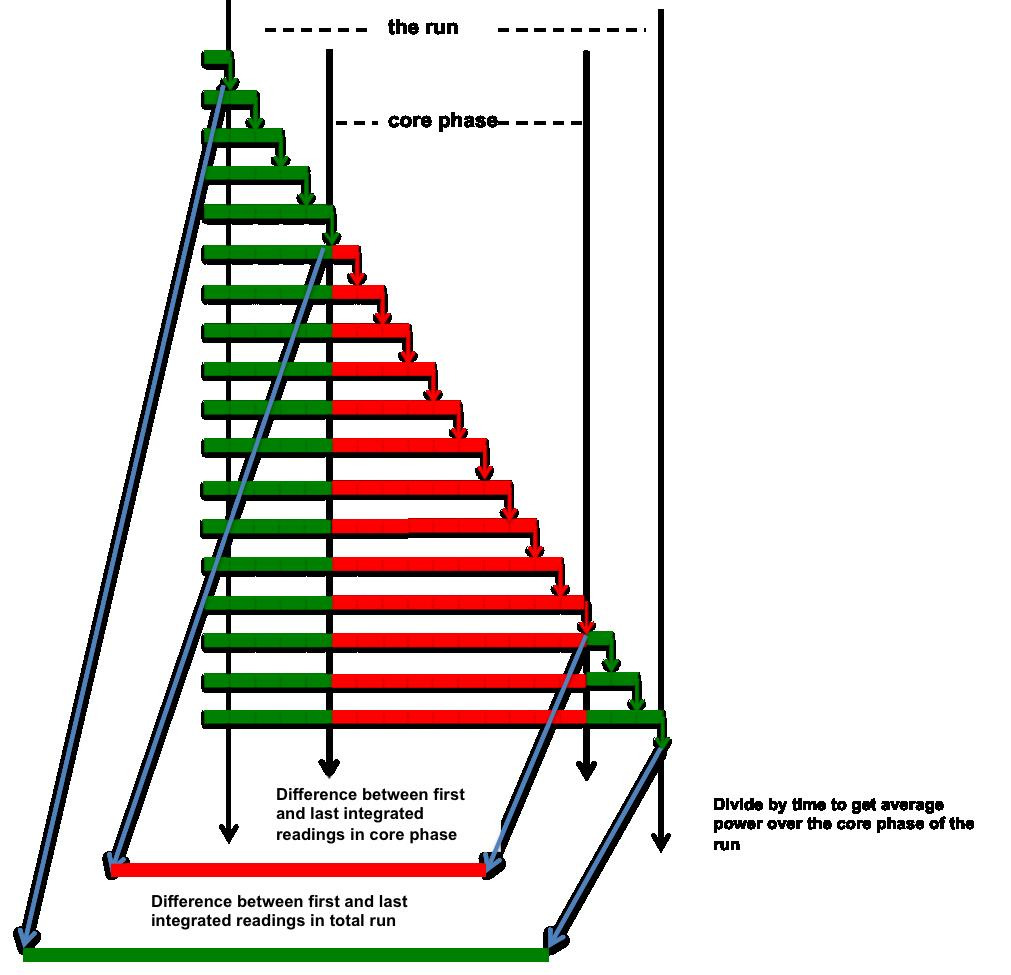
\includegraphics[width=4in]{fig3-5}
\caption{Aspect~1 of Level~3 Power Measurements}
\label{fig:a1l3pm}
\end{figure}

\section{Format of Reported Measurements}
\label{sec:FoRM}
\noindent
Levels 2 and 3 require the complete set of measurements. The submitter may choose to provide these values in a CSV file. Do not provide scans of paper documents.
\wl

\noindent
The submitter may find it useful to create a graph showing the power and energy during the workload as shown in Figure~\ref{fig:powengwl}. Keep this graph for reference, but do not provide it as part of the submission.


%INCLUDE FIG 3-6
\begin{figure}
\centering
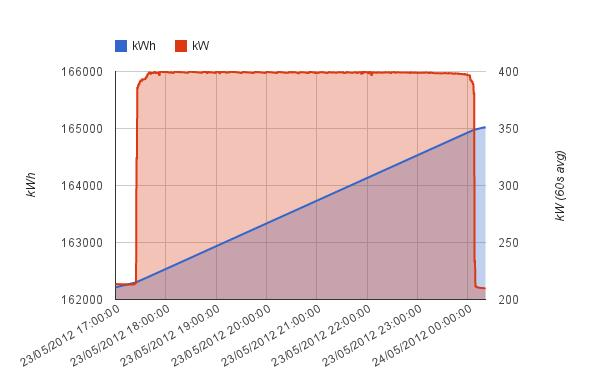
\includegraphics[width=4in]{fig3-6}
\caption{Power and Energy During the Workload}
(used with permission from Universit‚ Laval, Calcul Qu‚bec, Compute Canada)
\label{fig:powengwl}
\end{figure}

\section{Aspect 2: Machine Fraction Instrumented}
\label{sec:A2MFI}
\noindent
Aspect~2 specifies the fraction of the system whose power feeds are instrumented by the measuring equipment. 
\wl

\noindent
Level~3 requires that the entire machine be measured. Level~2 requires a higher fraction than Level~1.
\wl

\noindent
Levels 1 and 2 do not measure the power of the entire system, but require only a measurement of a fraction of the system and estimate the total power consumotion by extrapolation.
When calculating the average power of the full machine for Levels 1 and 2, the measured power must be divided by this fraction to 
extrapolate to the average power drawn by the whole machine. For example, if the submitter measures the power delivered 
to $ \frac{1}{4} $ of the machine, the submitter must then multiply the measured power by 4 to obtain the power for the whole machine.  
The higher machine fractions are required at the higher quality levels to reduce the effects of random fluctuations and minor differences in hardware influencing the power measurements.  The larger the sample, the more transients will tend to cancel out.
\wl

\noindent
The requirements with respect to the compute-node subsystem for each quality level are as follows.

\begin{itemize}
\item
L1: The largest of $\frac{1}{10}$ of the compute-node subsystem or at least 2~kW or 15 compute nodes. Alternatively, at least 40~kW or the entiry system.
\item
L2: The largest of $\frac{1}{8}$ of the compute-node subsystem or at least 10~kW or 15 compute nodes.
\item
L3: the power use of the whole machine must be measured.
\end{itemize}

\noindent
For measurements of other subsystems (network, storage, etc.), measure at least $\frac{1}{10}$ for Level~1, $\frac{1}{8}$ for Level~2, and everything for Level~3.
\wl

\noindent
The fraction of a subsystem that is measured must be chosen such, that the entire subsystem is a real multiple of the fraction.
For instance, a cluster consisting of blade servers with 8 nodes per chassis requires a measurement of entire chassis, hence a multiple of 8 nodes.
Even if individual node power could be measured, that would not be valid as it would not include the common chassis.
\wl

\noindent
The requirement for Level~1 and Level~2 include the measurement of at least 15 nodes.
For a cluster consisting of individual servers, a node is simply defined as one server.
There are architectures with multiple individual servers in one chassis, e.g. 2U twin or twin$^2$ servers with 2 and 4 servers per chassis and blade servers with many more nodes in one chassis.
Usually, all the nodes in one chassis share redundant power supplies.
In that case, you have to measure entire chassis, including all the power supplies of a chassis.
The measurement of a chassis is then considered a measurement of as many nodes as there are nodes in the chassis.
\wl

\noindent
For a measurement of only a fraction of a subsystem, this fraction must be chosen randomly.
In this context, random refers to the entity that are measured.
For instance, if you measure nodes then choose random nodes, if you measure entire racks, choose random racks.
It is not allowed to screen the system for components with lower power consumtion and then measure only that fraction nor is it allowed to replace components in the chosen fraction by ones with lower power consumption.
\wl

\section{Aspect 3: Subsystems Included in Instrumented Power}
\label{sec:A3SIiIP}
\noindent
Aspect 3 specifies the subsystems included in the instrumented power. 
\wl

\noindent
Subsystems in the context of this document are power subsystems. A power subsystem is that part of a supercomputer which can be measured in isolation for power consumption while the supercomputer is performing a task. 
\wl

\noindent
Subsystems include computational nodes, any interconnect network the application uses, any head or control nodes, any storage system the application uses, and any internal cooling devices (self-contained liquid cooling systems and fans).
\wl

\noindent
If some subsystems are part of the measured power, their power may not be subtracted out after the fact.  The explicitly measured value must be used as is.
\wl


\noindent
For Level~1, both the compute-node subsystem and the interconnect must be reported.  
The compute-node subsystem power must be measured. 
The interconnect subsystem participating in the workload must also be measured or, if not measured, the contribution must be estimated.
Include everything that you need to operate the interconnect network that is not part of the compute subsystem. 
This may include infrastructure that is shared, but excludes parts that are not servicing the system under test.
For some systems, it may be impossible not to include a power contribution from some subsystems. 
In this case, provide a list of the measured subsystems, but do not subtract an estimated value for the included subsystem. 
\wl

\noindent
For Level~2, include the compute node subsystem.
Other subsystems participating in the workload must be measured or estimated.
\wl

\noindent
For Level~3, all power going to the parts of a computer system that participate in a workload must be included in the power measurement. 
The reported power measurement must include all computational nodes, any interconnect network the application uses, any head or control nodes, any storage system the application uses, all power conversion losses inside the computer, and any internal cooling devices (self-contained liquid cooling systems and fans).  
\wl

\noindent
For Levels 1 and 2, estimations of other subsystems besides the compute subsystem must be performed by substituting the measurement by an uppower bound derived from the maximum specified power consumption of all hardware components.
\wl

\noindent
For Levels 2 and 3, the reported power measurement may exclude storage subsystems that don't participate in the workload. It is not required to exclude such storage subsystems. However, if these storage subsystems are part of the cabinet or rack being measured, they may not be excluded even if they are not used. That is, the submitter cannot calculate their contribution and subtract that contribution. If the storage subsystem is not part of the rack or cabinet being measured and it does not participate in the workload, it need not be measured.
\wl

\noindent
In some cases, the submitter may be measuring power that the application doesn't actually use. If the submitter can exclude the unused subsystems from the measurement or easily turn off the power to the unused subsystems, then the submitter can choose not to include those subsystems in the measurement. 
\wl

\noindent
For example, the node board may include compute nodes and GPUs, and the application may not actually use the GPUs.  If you cannot easily shut down the GPUs (say with an API), you must still include the power that they use. It is not acceptable to measure the power for both the compute nodes and the GPUs and then subtract the GPU power from the measurement.
\wl

\noindent
A site may include more subsystems than are strictly required if it chooses or if it is advantageous from a measurement logistics point of view.  
\wl

\noindent
A particular system may have different types of compute nodes. The system may have compute nodes from different companies or even compute nodes with different architectures. These compute nodes are said to belong to different heterogeneous sets.
\wl

\noindent
With Level~3, the submitter need not be concerned about heterogeneous sets of compute nodes because Level~3 measures the entire system. 
\wl

\noindent
Levels 1 and 2, however, measure a portion of the compute-node subsystem and estimate contributions from unmeasured portions. With Levels 1 and 2, the submitter must measure at least one member of each heterogeneous set. The submitter must include a power measurement from at least one compute node in each heterogeneous set and then estimate the contribution from the remaining members of the set. 
\wl

\noindent
For example, assume there exist two sets of compute nodes, a set called A and another called B.  The submitter is able to measure the power 
consumed by $ \frac{1}{2} $ of the A compute nodes and $ \frac{1}{4} $ of the B compute nodes.
\wl

\noindent
The total power measurement reported for compute nodes would then be 

\noindent
\[ Total~power=2*(power~from~compute~nodes~A) 
                              + 4*(power~from~compute~nodes~B) \]

\noindent
The assumption of Levels 2 and 1 is that all the compute nodes in a set react identically to the workload.


\section{Aspect 4: Instrumentation Location where the Electrical Measurements are Taken}
\label{sec:A4wEMaT}
Aspect 4 specifies where in the power distribution system the power delivery is measured.  For all quality levels, the submission indicates where power is measured and the quantity of parallel measurements.
\wl

\noindent
Measurements of power or energy are typically made at multiple locations in parallel across the computer system. For example, such locations can be at the entrance to each separate rack, or at the output connector of multiple building transformers. 
\wl

\noindent
All the reported measurements taken in parallel at a given instant in time are then summed into a total measurement for that time.  The total measurement for a given moment in time constitutes one entry in the series of measurements that becomes part of the submission.
\wl

\noindent
AC measurements are upstream of the system's power conversion. If the measurements are in a DC context, the submitter may have to take into account some power loss. 
Refer to Section~\numnameref{sec:AfPL}.
\wl

\noindent
Electrical power or energy measurements shall be taken in one of the following locations.

\begin{itemize}
\item[{A)}]
At a location upstream of where the electrical supply from the data center is delivered to the computer system

OR

\item[{B)}]
At the location of the electrical supply delivery to the computer system from the data center

OR

\item[{C)}]
At a location just inside of the computer system that is electrically equivalent to location B) above.  This includes the following. 

\begin{itemize}
\item
At any location within a passive PDU, at the input to the PDU, at the output connector(s) of the PDU, or anywhere in between 
\item
At the input connector to the first power-modifying component (for example, the Blue Gene bulk power module, Cray AC/DC converters, and possibly the input connector to one or more crate power supplies)
\end{itemize}
\end{itemize}

\noindent
If the measuring device or devices used to satisfy Aspect 1 also meet the ABC location requirements specified above, then those devices are sufficient to obtain the measurements needed for submission.
\wl

\noindent
Refer to Section~\ref{sec:MDSpecs} for the specifications of the required accuracy of the power meter devices.

\subsection{Adjusting for Power Loss}
\label{sec:AfPL}
\noindent
If the measurement device(s) that satisfy Aspect 1 are downstream of the ABC locations specified above, then two sets of measurements must be taken in order to determine the power loss between the required and the actual measurement location. 

\begin{itemize}
\item
For a Level~1 measurement, the power loss may be a load-varying model based on specifications from the manufacturer.  
\item
For a Level~2 measurement, the power loss may be a load-varying model based on an actual physical measurement of one power supply in the system.  
\item
For a Level~3 submission, the power loss must be measured simultaneously by a device at the required location (one of the ABC locations) measured at least once every five minutes, averaged long enough to average out the AC transients. 
\end{itemize}

\noindent
For all three levels, the power losses used and how they were determined must be part of the submissions.

\subsection{Data Center Schematic}
\noindent
Figure~\ref{fig:powmeasschem} is an example of a simple power measurement schematic. This example shows only one power measurement location.
\wl


\noindent
Submitters may find it useful to create such a schematic to identify the power measurement locations. Keep this schematic for reference, but do not provide it as part of the submission.

%INCLUDE FIG 3-7
\begin{figure}
\centering
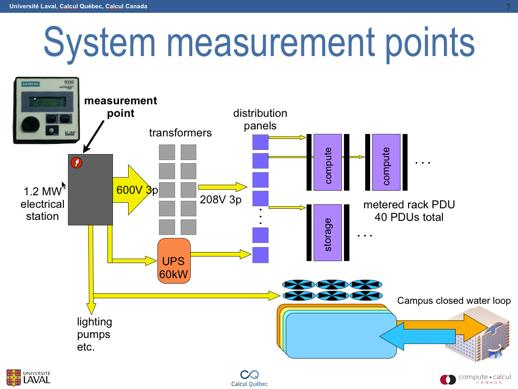
\includegraphics[width=4in]{fig3-7}
\caption{Example of a Power Measurement Schematic}
(used with permission from Universit\'{e} Laval, Calcul Qu\'{e}bec, Compute Canada)
\label{fig:powmeasschem}
\end{figure}


\section{Environmental Factors}
\label{sec:EF}
\noindent
Reporting information about the cooling system temperature is optional.
It is requested to provide a description of the cooling system as well as where and how the temperature was measured.
Reporting temperature allows for better comparison of reported results, as there is a indirect correlation between temperature and power.

\wl

\noindent
All other environmental data is optional. 
Other environmental data may include factors such as:

\begin{packed_item}
\item[{-}]
\% deviation between supply and rated voltage and frequency (recommended $\pm$\,5\%)
\item[{-}]
\% total harmonic distortion (recommended \textless\,2\% THD )
\item[{-}]
line impedance (recommended \textless\,0.25 ohm)
\item[{-}]
relative humidity
\end{packed_item}

